% 04_bench_exp.tex - VKIG-Bench + Experiments (v2 rewrite of old draft Sections 5-6).
% Pure body fragment. Assumes the preamble loads: booktabs, amsmath, amssymb,
% graphicx, natbib, pgfplots (\pgfplotsset{compat=1.18}).
% Companion appendix fragment: 92_appendix_tables.tex (labels app:e2e, app:cross,
% app:decomp, app:grid, app:judge, app:cost).

\section{VKIG-Bench}\label{sec:bench}

\paragraph{Why a new benchmark.}
MRAMG-Bench \citep{mramgbench2502} and similar interleaved-generation benchmarks evaluate factual image generation but contain no video and no keyframe-provenance dimension; V-STaR \citep{vstar2503} has video and bounding boxes but scores question answering rather than generated images. VKIG-Bench couples video provenance, newly generated images, and keyframe consistency, and thereby measures whether the images an answer displays are traceable to and consistent with a source frame. This is also the axis on which unified models \citep{bagel2505,showo22506} remain untested (Section~\ref{sec:exp-unified}).

\paragraph{Evaluation dimensions.}
VKIG-Bench scores six dimensions: text correctness (LLM-judge accuracy), image-text consistency (VQAScore \citep{vqascore}), keyframe consistency between the generated image and its source-keyframe object (DreamSim and DINO similarity), spatio-temporal localization (temporal IoU over timestamps and spatial IoU over boxes), image quality (FID and KID), and an overall human A/B win rate. The first two and the last two are standard; keyframe consistency and spatio-temporal localization are, to our knowledge, not scored together by any existing benchmark.

\paragraph{Data sources and construction.}
The labeled backbone converts the V-STaR seed \citep{vstar2503}, 2{,}094 fully public videos with 16{,}793 boxes and when-where-what reasoning chains, into the benchmark format. A self-built film and short-drama portion uses subtitle extraction, OCR, and Grounding-DINO pseudo-boxes, produced semi-automatically with human spot checks; box-free sources receive pseudo-boxes that are flagged as such, with a human-verified subset. Each sample stores the video, the query, the gold answer text, and gold evidence (keyframe timestamp, bounding box, object, and a reference image), together with the pseudo-box flag. We start at 300 to 500 samples (dev 100, test 300 or more) and plan growth to 1k--2k; Open-o3-Video \citep{openo3video2510} may seed stronger supervision once its release is confirmed. Construction proceeds by extracting query-driven keyframes from the raw video, grounding the target object, deriving a gold reference image from the grounded region, and storing the record after a human spot check of box and image correctness.

\section{Experiments}\label{sec:exp}

\subsection{Setup}\label{sec:exp-setup}

The Understand Agent uses Qwen3-VL \citep{qwen3vl2511}, which reads long video natively with frame timestamps. The Generation Agent uses FLUX.1-dev or FLUX.1 Kontext-dev with OminiControl \citep{ominicontrol2411}, or Qwen-Image-Edit; open-vocabulary detection uses Grounding-DINO or APE \citep{videorag2411}; text embeddings use BGE-M3. All runs below fit on a single RTX 4090D 24GB GPU, with larger runs on an A100-80G. The main pipeline is training-free; the optional LoRA variant fits in 16--18GB with gradient checkpointing at $512^2$ resolution and an 8-bit optimizer. The main external comparison is Zero-Shot STVG \citep{zeroshotstvg2509}, bridged to our joint keyframe metric (Section~\ref{sec:exp-select}), and a unified-model control uses Janus-Pro-7B \citep{januspro2501} (Section~\ref{sec:exp-unified}). VideoRAG \citep{videorag2502}, Open-o3-Video \citep{openo3video2510}, M2RAG \citep{m2rag2411}, and M2IO-R1 \citep{m2ior12508} are cited as reference points but not run as baselines; comparisons against BAGEL \citep{bagel2505} and Show-o2 \citep{showo22506} are left to future work. Metrics follow Section~\ref{sec:bench}.

\subsection{End-to-end runs and the temporal bottleneck}\label{sec:exp-e2e}

\paragraph{A real-video trace.}
We first ran the full five-stage pipeline on a real V-STaR street-scene clip (id 7771650716) with the query ``what walks in front of a man in white?'' and target object dog, on a single RTX 4090D. From 61 frames the selector chose $t=3.0$\,s (a man walking a dog, keyframe score 0.261); Qwen3-VL answered correctly (``a brown dog walks in front of the man in white''); an early SDXL-Turbo run generated a new image of a brown dog on the street; the keyframe was a temporal hit with subject CLIP similarity 0.673 and CLIP text alignment 0.285. Grounding-DINO-base, however, mislocalized the small, distant dog (box on empty ground, confidence 0.49, IoU 0), a failure only real data exposes. Replacing the detector with Qwen3-VL's native grounding corrected this on the same sample, raising spatial IoU from 0.0 to 0.363. The full trace appears in Appendix~\ref{app:e2e}.

\paragraph{V-STaR development subset.}
We report localization jointly: a keyframe counts as correct only if its timestamp falls in the gold temporal window and its box matches the gold box at the stated IoU threshold. A diagnostic spatial-only number (box against the nearest-in-time gold box) is also reported and is optimistic, since it ignores whether the moment is right. On the first 150 videos of the V-STaR test split, used as a development subset (all 150 completed; one primary keyframe per clip, grounding boxes in a 0--1000 normalized coordinate frame), the pipeline of object-conditioned keyframe selection, Qwen3-VL grounding, and SDXL-Turbo generation reaches joint accuracy 0.233 at IoU 0.3 and 0.213 at IoU 0.5, with temporal recall 0.26 and spatial IoU 0.72 when temporally correct; CLIP subject similarity is 0.66, CLIP text alignment 0.29, and the diagnostic nearest-frame IoU 0.39 (Appendix~\ref{app:e2e}). When the pipeline picks a keyframe at the right moment the box is accurate, but only 26\% of keyframes land in the gold window, so the open problem is temporal keyframe selection rather than the detector. A 50-video ablation shows that object-conditioned scoring mainly improves the quality of the chosen frame: query-relevance selection gives joint acc@0.3 0.24 with conditional IoU 0.69, adding temporal smoothing gives 0.22 and 0.56, and object conditioning gives 0.28 and 0.79 (Appendix~\ref{app:e2e}). On identical keyframes (query-relevance selection with smoothing), Qwen3-VL native grounding beats Grounding-DINO-base on the diagnostic spatial IoU (0.323 against 0.292) but not on the joint metric (acc@0.3 0.22 against 0.24); better boxes cannot fix timing. We adopt Qwen3-VL grounding for its box quality and single-model economy, and note that the 0.28 above uses object-conditioned selection, that is, different keyframes, so it is not a same-keyframe grounding comparison.

Two conventions matter for reading these numbers. The V-STaR grounding target is the benchmark's annotated object, an oracle-style input on object identity that deliberately isolates temporal and spatial localization from object naming; HC-STVG, the main dataset below, instead infers the object with a noun-phrase heuristic. The 1\,fps frame reader caps at 64 frames, so on the small fraction of V-STaR clips whose gold window falls after 64\,s a hit is structurally impossible, and the V-STaR numbers are a mild lower bound; HC-STVG clips last 20\,s and never reach the cap. The design components not activated in these runs (BGE-M3 pruning, the coverage term, and the shared-RAG feedback) are itemized in Section~\ref{sec:method}.

\paragraph{Cross-dataset confirmation.}
To test whether the finding is dataset-specific, we ran the same localization pipeline on HC-STVG v2, an independent human-annotated spatio-temporal grounding benchmark of 20\,s clips with per-frame person tubes and a natural-language description. We evaluate 1000 video-ready samples from a community mirror of the test split (six samples skipped for missing videos), taking the grounding target as the noun phrase before the caption's first verb (annotation subject field as fallback), a strict temporal hit (pad 0\,s), and the spatial gold as the tube box nearest in time to the predicted keyframe. Joint accuracy reaches 0.419 at IoU 0.3 and 0.396 at IoU 0.5, with temporal recall 0.524 and conditional spatial IoU 0.664; results are stable across scale, with acc@0.3 moving from 0.430 at $n=200$ to 0.419 at $n=1000$. Compared with V-STaR, temporal recall roughly doubles on these well-scoped clips while conditional box accuracy stays high, and the bottleneck ordering is identical on both datasets. Part of the recall gap is an instrument artifact: the 64-frame reader cap truncates long V-STaR clips but never the 20\,s HC-STVG clips, so removing it would narrow the measured gap without changing the ordering. The noun-phrase extractor returns an over-long phrase (more than 8 words) on about 29\% of samples (293/1000), which depresses these numbers. Samples whose grounding returns no box are counted as incorrect; grounding produces a box on 96.6\% of temporal hits, and scoring the excluded 18/524 as IoU 0 would change the conditional IoU from 0.664 to 0.641 while leaving the headline accuracies untouched. The full cross-dataset table and remaining conventions appear in Appendix~\ref{app:cross}.

\subsection{Isolating the bottleneck with selection-strategy baselines}\label{sec:exp-oracle}

To quantify how much of the localization score comes from content-based selection as opposed to a positional prior, we hold grounding fixed (Qwen3-VL) and swap only the selection step on the same 300 HC-STVG test clips. A seeded random frame scores acc@0.3 0.257; our object-conditioned CLIP selection scores 0.443; the video-midpoint frame, a strong positional prior on this temporally centred dataset, scores 0.440; and a temporal oracle that picks the frame nearest the gold interval's midpoint scores 0.787 (Appendix~\ref{app:decomp}). Content selection clearly beats chance, by 73\% relative over random. It only ties the trivial midpoint prior here, because HC-STVG action windows are centred; on street-scene V-STaR, object conditioning did help (Section~\ref{sec:exp-e2e}). The decisive number is the oracle: with grounding and box regression unchanged, perfect temporal selection alone would lift end-to-end localization from 0.44 to 0.79, which puts the selectable headroom at roughly $+0.34$ absolute and identifies temporal keyframe selection, not the detector, as the bottleneck. A decomposition of joint accuracy into temporal recall and conditional spatial precision, together with a gold-window tercile analysis, supports the same attribution (Appendix~\ref{app:decomp}).

\subsection{Main localization results}\label{sec:exp-select}

We evaluate the two-stage selector (Section~\ref{sec:method}) on the 282-clip common subset shared by our runs and the bridged baseline, holding grounding fixed and using identical denominators across all rows with the strict temporal pad of 0. The study above uses the fuller 300-clip set; oracle values are reported per denominator (0.787 at $n=300$, 0.780 at $n=282$).

\paragraph{Bridging protocol.}
The zero-shot STVG baseline \citep{zeroshotstvg2509} emits a spatio-temporal tube rather than a keyframe. We convert its output as follows: the keyframe timestamp is the midpoint of its predicted temporal interval, the predicted box is the tube box nearest that timestamp, and the gold box is the gold-tube box nearest the keyframe; scoring then uses exactly our joint metric, with strict pad 0 and missing boxes counted as incorrect. Because the midpoint falls between frames, we compute both roundings: floor gives temporal recall 0.642, acc@0.3 0.447, and acc@0.5 0.394; ceil gives 0.667, 0.443, and 0.390. Table~\ref{tab:selector} reports floor, the variant more favorable to the baseline on the headline acc@0.3, and E2 wins under both roundings. As a sanity anchor, our native-protocol reproduction of the baseline reaches m\_vIoU 0.221 over the full 299-clip reproduction run before intersecting to the 282-clip common set, consistent with a community-reported reproduction (0.207, filed in the official repository's issue tracker) and the paper's 0.236, so the bridged numbers rest on a faithful reproduction.

\begin{table}[t]
\centering
\small
\begin{tabular}{lccc}
\toprule
Selection ($n=282$, grounding fixed) & Temporal recall & acc@0.3 (joint) & acc@0.5 \\
\midrule
E0: object-conditioned scoring & 0.557 & 0.433 & 0.411 \\
E1: E0 + action-phrase channel & 0.610 & 0.489 & 0.468 \\
E2: two-stage (MLLM window $\rightarrow$ in-window selection) & 0.720 & 0.567 & 0.539 \\
\midrule
Zero-Shot STVG \citep{zeroshotstvg2509}, bridged (floor rounding) & 0.642 & 0.447 & 0.394 \\
Temporal oracle (upper bound) & 1.000 & 0.780 & -- \\
\bottomrule
\end{tabular}
\caption{Main localization results on the 282-clip HC-STVG v2 common subset, identical denominators and strict temporal pad 0. E1 and E2 are two independent modifications of E0, not a nested stack. The bridged baseline follows the protocol in Section~\ref{sec:exp-select} and is reported under its more favorable rounding.}
\label{tab:selector}
\end{table}

\paragraph{Results.}
E1 raises acc@0.3 from 0.433 to 0.489 and the two-stage E2 reaches 0.567 (Table~\ref{tab:selector}); the full factorial combination of the two modifications is left to future work. Box quality when temporally correct stays within 0.61--0.64 across E0, E1, and E2 on this subset (no-box counted as IoU 0), so the improvement is primarily associated with higher temporal recall: the conditional spatial IoU moves by at most 0.035 while temporal recall moves by $+0.16$, which is where the oracle study located the bottleneck. E2 changes which keyframe is grounded, so this is an association rather than a controlled causal decomposition. Against the bridged baseline, E2 is higher by $+0.121$ acc@0.3 on identical clips under the joint keyframe metric, and it requires no gradient-based test-time adaptation; the added cost is one MLLM call per clip, measured at $+1.46$\,s (Appendix~\ref{app:cost}). The remaining oracle gap is $0.780-0.567\approx 0.21$, down from roughly 0.35 at the same denominator; grid density, iterative window refinement, and audio or subtitle cues are natural next steps. As an exploratory check on leakage, Stage A receives only the sparse frame grid and the query text, and the gold interval is never passed to the model; among the 203 temporally correct predictions in the subset, the median keyframe distance to the nearest gold boundary is 1.76\,s, with no boundary-snapping signature. Stage-A raw window outputs were not persisted in this run, so a full audit of the MLLM responses is left to future work.

\paragraph{Scale and grid density.}
Re-running E2 with grid $g=10$ on 1000 HC-STVG test clips gives temporal recall 0.688, acc@0.3 0.540, and acc@0.5 0.517, against 0.524, 0.419, and 0.396 for E0 on the same clips; the improvement holds at scale, and the mild regression from the 300-clip subset is expected. Densifying the Stage-A grid improves both the window and the end metric up to $g=20$: grids of 10, 15, and 20 frames give temporal recall 0.717, 0.753, and 0.783 and acc@0.3 0.570, 0.603, and 0.627 at $n=300$, shrinking the oracle gap to about 0.16 at the peak, at the cost of proportionally more image tokens in the single Stage-A call. Beyond 20 frames the gains reverse: the curve is an inverted U, with $g=25$ at 0.580 and $g=30$ at 0.537, below even $g=10$. Packing more frames into one call dilutes the model's cross-frame temporal attention, so $g=20$ is the operating point and the coarse window cannot be densified for free. The full sweep with confidence intervals, and the disclosure of a selector bug that affected early $g\ge 15$ runs but no headline number, appear in Appendix~\ref{app:grid}.

\paragraph{Statistical significance.}
All point estimates carry 95\% bootstrap confidence intervals from 10k resamples (Appendix~\ref{app:grid}), and the two-stage gains are significant on paired tests over identical clips (Table~\ref{tab:sig}). E0 to E2 lifts acc@0.3 from 0.419 to 0.540 at $n=1000$ (McNemar $p<10^{-4}$; Wilcoxon on box IoU $p<10^{-4}$), and E2 also beats the strong midpoint prior at $n=300$ (0.440 to 0.570, McNemar $p=0.0006$). The E1 to E2 step is weaker ($+0.073$, McNemar $p=0.015$, Wilcoxon $p=0.079$, not significant), consistent with E1 and E2 being independent rather than nested modifications. Densifying the grid from $g=10$ to $g=20$ raises acc@0.3 ($+0.057$, McNemar $p=0.043$) while leaving per-sample box IoU statistically unchanged (Wilcoxon $p=0.90$); the decomposition in Appendix~\ref{app:decomp} attributes about 94\% of this gain to temporal recall. We leave the remaining ablations to future work: removing object conditioning, whole-frame conditioning, crop-only output, BGE-M3 pruning, the shared RAG, threshold sweeps, mixture weights, generator choice, condition ablation, and the full E1$\times$E2 factorial. Trained spatio-temporal grounding models and further video-RAG and interleaved-generation baselines \citep{videorag2411,m2rag2411} likewise remain future comparisons.

\begin{table}[t]
\centering
\small
\begin{tabular}{lccccc}
\toprule
Paired comparison (same clips) & acc@0.3 & $\Delta$ & McNemar b/c & McNemar $p$ & Wilcoxon (IoU) $p$ \\
\midrule
E0 $\rightarrow$ E2 ($n=1000$) & $0.419 \rightarrow 0.540$ & $+0.121$ & 61/182 & $<10^{-4}$ & $<10^{-4}$ \\
midpoint $\rightarrow$ E2 ($n=300$) & $0.440 \rightarrow 0.570$ & $+0.130$ & 42/81 & 0.0006 & 0.0001 \\
E1 $\rightarrow$ E2 ($n=300$) & $0.497 \rightarrow 0.570$ & $+0.073$ & 27/49 & 0.015 & 0.079 (n.s.) \\
E2 $g10 \rightarrow g20$ ($n=300$) & $0.570 \rightarrow 0.627$ & $+0.057$ & 23/40 & 0.043 & 0.90 (n.s.) \\
\bottomrule
\end{tabular}
\caption{Paired significance tests over identical clips. b/c denotes discordant pairs (first-only-correct / second-only-correct).}
\label{tab:sig}
\end{table}

\subsection{Keyframe faithfulness}\label{sec:exp-faith}

\paragraph{Protocol.}
We call a generated image \emph{semantically faithful} to its source keyframe if it depicts the same moment: the same person or persons, clothing, pose and action, and scene layout, with an emotional expression consistent with the source. A crying face rendered as smiling is a violation; a micro-level facial redraw without an emotion change is not (a refinement introduced in Round 3). Lighting, color, and style changes are permitted, and identity-level pixel fidelity is out of scope, consistent with the task motivation in Section~\ref{sec:intro}. We evaluate with human annotation (one author, binary labels plus an unsure option) and with an MLLM judge (Qwen3-VL, prompted with the two images and asked strictly for a same-moment judgment in JSON).

\paragraph{Round 1: permissive baseline ($n=40$).}
FLUX.1-Kontext-dev conditioned on E2-selected keyframes with a permissive instruction (``re-render as a cinematic promotional poster shot, dramatic lighting'') is humanly faithful on 12/40 pairs (30\%). The MLLM judge passes 4/40; agreement with the human is 31/39 (79.5\%, excluding one unsure), and the judge accepts none of the 27 pairs the human rejected, making it a conservative candidate gate pending held-out validation. Human-categorized failures fall into wholesale re-imagination (the scene replaced entirely, for example an outdoor group scene regenerated as a studio portrait of one man), clothing or identity drift, and over-darkening from the dramatic-lighting token. CLIP subject similarity averages 0.60 on the same images, a reassuring mean that conceals 70\% unfaithful outputs: CLIP does correlate with the human label (AUC 0.846, Mann-Whitney $p=0.001$; faithful mean 0.72 against unfaithful 0.55) but admits no usable threshold, with 72\% of pairs inside the class-overlap band $[0.45, 0.76]$ and the best single cutoff still misclassifying 6/39. A metric that ranks yet cannot gate is precisely why a dedicated protocol is needed. Full Round-1 tables are in Appendix~\ref{app:judge}.

\paragraph{The automatic-metric family degrades together.}
To test whether CLIP's behavior is idiosyncratic, we computed three further standard image-similarity metrics on the same 80 keyframe-generation pairs (40 permissive, 40 constrained) and scored each against the human labels (Table~\ref{tab:metricfamily}). Every metric's mean moves in the faithful direction under content-locking, and every metric ranks well in the permissive regime, yet all four lose discriminative power in the constrained regime, where the residual failures are expression-level. DreamSim and DINOv2 are the strongest rankers in both regimes but are not exempt from the degradation. The finding is therefore a family-wide property rather than a CLIP quirk: appearance-level automatic metrics separate wholesale re-imagination from faithful renders, yet none of them can adjudicate the subtle failures that remain once content is locked, which is exactly the regime a deployed system operates in.

\begin{table}[t]
\centering
\small
\begin{tabular}{lccc}
\toprule
Automatic metric & mean, permissive $\rightarrow$ constrained & AUC (permissive) & AUC (constrained) \\
\midrule
DreamSim $\downarrow$ & $0.535 \rightarrow 0.377$ & 0.873 & 0.756 \\
DINOv2 CLS cosine $\uparrow$ & $0.388 \rightarrow 0.701$ & 0.870 & 0.766 \\
CLIP subject sim $\uparrow$ & $0.601 \rightarrow 0.708$ & 0.846 & 0.673 \\
LPIPS $\downarrow$ & $0.661 \rightarrow 0.557$ & 0.719 & 0.640 \\
\bottomrule
\end{tabular}
\caption{Four automatic metrics against human faithfulness labels on the same $2{\times}40$ pairs ($\downarrow$ distance, lower is closer; $\uparrow$ similarity). All four rank well under permissive prompting and all four degrade once failures become expression-level under constrained prompting.}
\label{tab:metricfamily}
\end{table}

\paragraph{Round 2: instruction-constrained A/B ($n=10$).}
Replacing the instruction with an explicit preservation constraint (``enhance this exact frame\ldots{} STRICTLY KEEP the same people, faces, clothing, poses and scene layout; only improve lighting/color/sharpness; keep bright; no text'') on the same 10 keyframes moves human faithfulness from 1/10 (10\%) to 10/10 (100\%); the MLLM judge passes 0/10 and 3/10 respectively (Appendix~\ref{app:judge}). In this matched sample, unfaithfulness behaves as an instruction-constraint problem rather than a hard capability ceiling, with the caveat that $n=10$ and capability limits at scale remain untested; our protocol is what makes this dimension measurable.

\paragraph{The faithfulness-artistry frontier.}
We added a second human-rated axis, \emph{poster-likeness} (1 = looks like a screenshot, 2 = some polish, 3 = looks like a real poster), and rated four instruction tiers on the same 10 keyframes; tiers A, B, and C were rated tier-blind in one shuffled session (30 pairs), and tier D was added later as a separate 10-pair batch. Once content is locked, poster-likeness rises from 1.10 (tier B) through 1.20 (C) to 1.50 (D) while faithfulness holds at 90--100\% (Table~\ref{tab:frontier}). Text instructions therefore recover some polish, but even the maximally artistic tier D plateaus at 1.50, well short of the 2.50 reached only when content is unlocked at 10\% faithfulness. Within a single call the two axes compose only partway, a bounded negative result at $n=10$ with one annotator.

If the single-instruction budget is zero-sum, decoupling content-locking from style-amplification should recover the frontier, so we instantiated both designed decoupling routes on the same 10 keyframes with shuffled joint annotation. The single-call constraint budget resets across calls: pass 1 locks content, and the image handed to pass 2 carries that content, so the second instruction can spend its full budget on style. Sequential two-pass editing (a tier-D content-locked edit followed by a pure style-amplification edit) reaches 10/10 faithful at poster-likeness 1.90 on the same keyframes, the first point beyond the single-call plateau. The chain then saturates: three- and four-pass variants stay at 1.90 (8/10 and 10/10 faithful), since by pass 2 the style instruction's content is fully absorbed. Parallel arms preserve exactly the modality their anchor encodes. IP-Adapter conditioning at scales 0.75 and 0.95 transfers the clip's gist (setting, palette, cast type) but never the moment (0/10 at both scales, poster-likeness 1.60). ControlNet-depth conditioning keeps the composition skeleton and reaches 2.30, the highest artistry of any anchored arm and close to the unlocked 2.50, yet re-imagines all appearance (0/10). The residual gap between 1.90 and 2.30 or 2.50 is appearance-preserving stylization, which no single anchor provides; composing anchors (pixel identity, geometric layout, and free style text) is the natural next design. All frontier measurements use $n=10$ per arm with a single annotator; chained passes inherit earlier-pass biases, and arm tags were visible in the annotation ids, as in prior rounds. Figure~\ref{fig:frontier} maps every evaluated protocol on the two axes.

\begin{table}[t]
\centering
\small
\begin{tabular}{llcc}
\toprule
Group & Protocol & Human faithful & Poster-likeness (1--3) \\
\midrule
Single instruction & A: permissive & 1/10 (10\%) & 2.50 \\
 & B: maximally constrained & 10/10 (100\%) & 1.10 \\
 & C: content locked, lighting freed & 9/10 (90\%) & 1.20 \\
 & D: content locked, artistry maximized & 9/10 (90\%) & 1.50 \\
 & D at scale ($n=40$, Round 3) & 28/40 (70\%) & 1.78 \\
\midrule
Sequential & two-pass editing & 10/10 (100\%) & 1.90 \\
 & three-pass & 8/10 (80\%) & 1.90 \\
 & four-pass & 10/10 (100\%) & 1.90 \\
\midrule
Parallel & IP-Adapter, scale 0.75 & 0/10 (0\%) & 1.60 \\
 & IP-Adapter, scale 0.95 & 0/10 (0\%) & 1.60 \\
 & ControlNet-depth & 0/10 (0\%) & 2.30 \\
\bottomrule
\end{tabular}
\caption{Faithfulness and poster-likeness across single-instruction tiers, sequential multi-pass editing, and parallel conditioning arms, all on the same keyframes ($n=10$ per row unless noted). Two-pass editing extends the single-instruction frontier on both axes, deeper chains saturate at 1.90, and each parallel anchor preserves only the modality it encodes.}
\label{tab:frontier}
\end{table}

\begin{figure}[t]
\centering
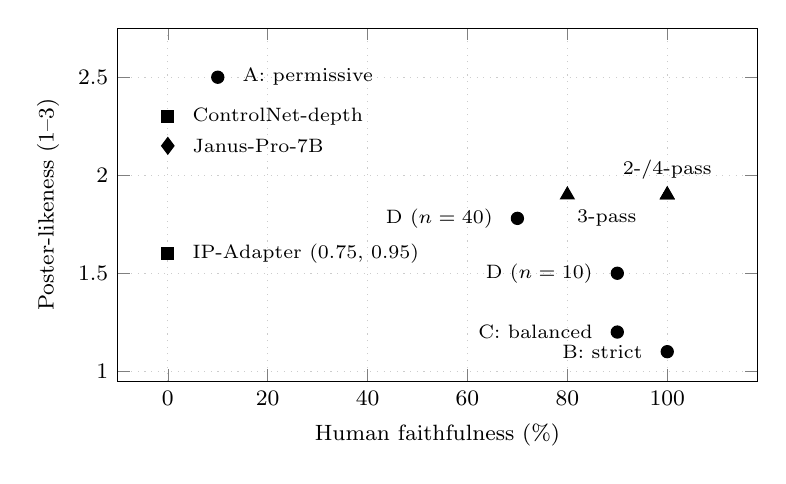
\begin{tikzpicture}
\begin{axis}[
    width=0.8\textwidth,
    height=0.5\textwidth,
    xlabel={Human faithfulness (\%)},
    ylabel={Poster-likeness (1--3)},
    xmin=-10, xmax=118,
    ymin=0.95, ymax=2.75,
    xtick={0,20,40,60,80,100},
    grid=major,
    grid style={dotted,gray!40},
    tick label style={font=\footnotesize},
    label style={font=\footnotesize},
]
\addplot[only marks, mark=*, mark size=2.2pt] coordinates {(10,2.50) (100,1.10) (90,1.20) (90,1.50) (70,1.78)};
\addplot[only marks, mark=triangle*, mark size=2.8pt] coordinates {(100,1.90) (80,1.90) (100,1.90)};
\addplot[only marks, mark=square*, mark size=2.2pt] coordinates {(0,1.60) (0,1.60) (0,2.30)};
\addplot[only marks, mark=diamond*, mark size=3.0pt] coordinates {(0,2.15)};
\node[font=\scriptsize, anchor=west] at (axis cs:13,2.50) {A: permissive};
\node[font=\scriptsize, anchor=east] at (axis cs:97,1.10) {B: strict};
\node[font=\scriptsize, anchor=east] at (axis cs:87,1.20) {C: balanced};
\node[font=\scriptsize, anchor=east] at (axis cs:87,1.50) {D ($n=10$)};
\node[font=\scriptsize, anchor=east] at (axis cs:67,1.78) {D ($n=40$)};
\node[font=\scriptsize, anchor=south] at (axis cs:100,1.93) {2-/4-pass};
\node[font=\scriptsize, anchor=north west] at (axis cs:80,1.87) {3-pass};
\node[font=\scriptsize, anchor=west] at (axis cs:3,1.60) {IP-Adapter (0.75, 0.95)};
\node[font=\scriptsize, anchor=west] at (axis cs:3,2.30) {ControlNet-depth};
\node[font=\scriptsize, anchor=west] at (axis cs:3,2.15) {Janus-Pro-7B};
\end{axis}
\end{tikzpicture}
\caption{Faithfulness against poster-likeness for the twelve evaluated protocols, all rated by the same annotator. Circles: single-instruction tiers A to D ($n=10$ each) and the tier-D Round-3 run at $n=40$ (Table~\ref{tab:frontier}). Triangles: sequential chains of two to four passes ($n=10$ each). Squares: parallel IP-Adapter arms at scales 0.75 and 0.95 and the ControlNet-depth arm ($n=10$ each). Diamond: the Janus-Pro-7B unified control ($n=20$, Section~\ref{sec:exp-unified}). The two-pass and four-pass chains coincide at (100, 1.90), and the two IP-Adapter scales coincide at (0, 1.60). Sequential editing extends the single-instruction frontier on both axes, while the parallel and unified arms, which lack pixel-level anchoring to the keyframe, sit at zero faithfulness regardless of artistry.}
\label{fig:frontier}
\end{figure}

\paragraph{Round 3: the best tier at scale ($n=40$).}
Applying the tier-D instruction to all 40 E2-selected keyframes (same keyframes and denominator as Round 1) yields 28/40 (70\%) human faithfulness against the permissive baseline's 12/40 (30\%), with mean poster-likeness 1.78; the 10-pair probe's 90\% and 1.50 reflect small-sample optimism. The annotation standard was sharpened for this round as stated in the protocol: an emotional expression contradicting the source moment counts as unfaithful, while facial redraw without an emotion change does not. CLIP subject similarity rises to 0.708 (from 0.601 permissive), but its discriminative power collapses in this regime: AUC drops from 0.846 to 0.673 ($p=0.087$, no longer significant), because the failures here are expression-level rather than wholesale and CLIP cannot see them. The MLLM judge passes 32/40, agrees with the human on 30/40 (75\%), and accepts 7 pairs the human rejected, so its zero-false-accept behavior from Round 1 does not transfer to the constrained regime; Cohen $\kappa$ is 0.34 against 0.41 in Round 1. Automatic proxies, both the metric family above and the judge, become less reliable exactly as the failures become subtler, so the human protocol remains the stable anchor and any automatic gate needs held-out validation before automated use. Round comparisons, the CLIP regime analysis, and the confusion matrices appear in Appendix~\ref{app:judge}.

\paragraph{Cost.}
On 20 clips with a single RTX 4090D, the E0 pipeline averages about 2.31\,s per clip and the E2 pipeline about 3.77\,s; the added 1.46\,s comes entirely from the Stage-A window call, with no gradient computation, in contrast to the per-sample test-time tuning of the zero-shot STVG baseline. One-time model loading takes 16.3\,s for CLIP plus 10.4\,s for Qwen3-VL. The stage-level breakdown is in Appendix~\ref{app:cost}.

\subsection{Unified-model control}\label{sec:exp-unified}

The hypothesis from Section~\ref{sec:intro}, that a single unified model does not replace the localization-grounded pipeline, receives a first instantiation here. Janus-Pro-7B \citep{januspro2501}, a unified understanding and generation model, receives an 8-frame uniform grid of the clip plus the query, describes the queried moment, and then generates the answer image from its own description, since the model offers no image-conditioned generation. Its outputs carry no timestamp and no bounding box: the localization protocol is structurally absent rather than merely unmeasured, and we record this per sample. The control uses the same 20 HC-STVG clips, the same human protocol, and the same annotator as Section~\ref{sec:exp-faith}.

\begin{table}[t]
\centering
\small
\begin{tabular}{lcc}
\toprule
Measure ($n=20$) & Janus-Pro-7B (unified control) & Ours (best tier D) \\
\midrule
Human faithfulness & 0/20 (0\%) & 28/40 (70\%) \\
Poster-likeness (1--3; stylization only) & 2.15 & 1.78 \\
Temporal localization output & none (structural) & keyframe timestamp, IoU-evaluated \\
Spatial localization output & none (structural) & bounding box, IoU-evaluated \\
\bottomrule
\end{tabular}
\caption{Unified-model control against the best-tier pipeline. The poster-likeness scale rewards surface stylization and does not penalize content deformation.}
\label{tab:unified}
\end{table}

The poster-likeness of 2.15 must be read with its scale in mind: the scale rewards surface stylization, such as cinematic grading and collage layouts, and does not penalize content deformation. The unified model's outputs score high on stylization while being anatomically and scenically deformed throughout (the annotator reports duplicated heads, warped bodies, and invented scenes), and none of the twenty depicts the actual moment; subjects are re-imagined wholesale. On the faithfulness-artistry map (Figure~\ref{fig:frontier}) the monolith lands in the same corner as permissive prompting: style without provenance. Without explicit localization and keyframe binding, nothing anchors generation to the real clip, and the failure cannot even be audited, because the model reports no when or where. These results cover one 7B unified model under one protocol, with 20 clips and a single annotator, and stronger unified models or richer prompting may narrow the stylization gap. We leave controls with BAGEL \citep{bagel2505} and Show-o2 \citep{showo22506} to future work, noting that the missing when-and-where output is a property of the architecture rather than of scale, and it is precisely what VKIG-Bench measures.
